\documentclass[oneside,senior,etd]{BYUPhysForDegree}

\usepackage[utf8]{inputenc}
\usepackage{rotating} 

\usepackage[russian]{babel}
\usepackage{amsfonts} % Пакеты для математических символов и теорем
\usepackage{amstext}
\usepackage{amssymb}
\usepackage{amsthm}
\usepackage{amsmath}
\usepackage{graphicx} % Пакеты для вставки графики
\usepackage{subfig}
\usepackage{color}
\usepackage{caption}
\usepackage{booktabs} % Для использования красивых линий таблицы
\usepackage[unicode]{hyperref}
\usepackage[nottoc]{tocbibind} % Для того, чтобы список литературы отображался в оглавлении
\usepackage{algorithmic} % Для записи алгоритмов в псевдокоде
\usepackage{algorithm}
\usepackage{adjustbox}
\usepackage{verbatim} % Для вставок заранее подготовленного текста в режиме as-is
\usepackage{listings}
\usepackage{wrapfig}
\usepackage{xcolor}
\usepackage{colortbl}
\usepackage{tabularx}
\usepackage{bbm}
\usepackage{subcaption}

\usepackage{commath}
\newcommand\Tau{\mathcal{T}}
\newcommand{\R}{\mathbb{R}}
\usepackage{color}
\usepackage[colorinlistoftodos, prependcaption]{todonotes}
\usepackage{multirow}
\newcommand*{\MyIndent}{\hspace*{0.2cm}}%

\Chair{Кафедра алгоритмических языков}
\Lab{~}
\Year{2024}
  %\Month{Июнь}
  \City{Москва}
  \AuthorText{Автор}
  \Author{Грибов Илья Юрьевич}
  %\AuthorEng{Gribov Ilia}
  \AcadGroup{424}
  % Если вы не Пупкин Василий Иванович, то скопируйте себе этот проект через меню и уже потом правьте
  \TitleTop{Оптимизация порождения состязательных примеров}
  %\TitleMiddle{}
  \TitleBottom{в задаче классификации} % leave empty if you don't need it
  %\TitleTopEng{Research and development of machine learning methods}
  %\TitleBottomEng{} % leave empty if you don't need it  
  %\docname{Курсовая работа}
  \docname{Выпускная квалификационная работа}
  %\docname{Магистерская диссертация}
  \Advisor{Лукашевич Наталья Валентиновна}  
  \AdvisorDegree{д-р техн. наук}
  %\Consultant{}
  %\ConsultantDegree{}
  
\Abstract{

\textbf{Состязательные примеры} - это данные, которые специально создаются или изменяются с целью нарушить работу алгоритма машинного обучения. Этот подход становится все более важным в контексте развития искусственного интеллекта, поскольку он позволяет проверять устойчивость и надежность алгоритмов в различных областях, таких как компьютерное зрение и обработка естественного языка.

В данной работе рассматриваются подходы, основанные на интерпретации прогнозов модели и анализе их внутренней структуры, к оптимизации процесса порождения состязательных примеров для задачи классификации текстов. В процессе работы было проведено сравнение различных подходов оптимизации и их влияния на итоговую генерацию. Промежуточные метрики и результаты сопровождаются иллюстрационными примерами. Результаты исследования могут быть применены для повышения устойчивости и надежности классификационных текстовых моделей и аугментации данных в области обработки текстов.

}
% \AbstractEng{Abstract}


%%%% DON'T change this. It is here because .sty does not support cyrillic cp properly %%%%
\University{Московский государственный университет имени М.В.Ломоносова}
\Faculty{Факультет вычислительной математики и кибернетики}
\GrText{гр.}
\AdvisorText{Научный руководитель}
\ConsultantText{}
\AbstractText{Аннотация}

\begin{document}
\fixmargins
\makepreliminarypages

\oneandhalfspace

\tableofcontents

\section{Введение}
\label{sec:Chapter0} \index{Chapter0}

\hspace{0.6cm}Большие нейронные модели NLP, в первую очередь BERT/GPT-подобные модели \cite{general1}, \cite{general2}, получили широкое распространение как в исследованиях, так и в промышленности, ввиду установленной зависимости между размером модели и ее результативностью при  решении задач. Однако как следствие, подобные модели обычно рассматриваются в виде некоторого \textbf{"чёрного ящика"}. Поэтому растёт озабоченность работой и надёжностью данных моделей, так как подобные системы часто принимают участие при принятии решений в различных сферах, где цена ошибки очень высока.

Зачастую невозможно учесть все виды отказов и проблем, которые могут возникнуть при эксплуатации данных моделей, поэтому оценка качества также должна проводиться с помощью модельных пояснений. Предоставление этих пояснений часто является основной мотивацией для понятия \textbf{“интерпретируемости”} моделей машинного и глубокого обучения. То есть, когда модели выдают неверный результат или их поведения начинает отклоняться от стандартного и первоначального задуманного, возникает необходимость в объяснениях, почему модель приняла то или иное решение на основе полученных входных данных. На сегодняшний день существует немало способов, которые могут позволить изучить поведение модели. Таковыми могут быть \textbf{состязательные примеры}.

\textbf{Состязательные примеры} - это специально подобранные входные данные, которые могут ввести в заблуждение или заставить ошибиться модель. В области обработки естественного языка (NLP) состязательные примеры могут быть созданы различными методами, такими как перефразирование текста, вставка опечаток, добавление отвлекающих элементов или замена слов синонимами. Цель состязательных примеров в NLP - проверить и улучшить устойчивость и надёжность моделей глубокого обучения. В данной работе в дальнейшем будут рассмотрены уже существующие на сегодняшний момент методы генерации состязательных примеров для текстов.

Также наряду с понятием состязательных примеров вводится понятие \textbf{состязательная устойчивость} — это мера восприимчивости модели к состязательным примерам. Её часто измеряют, используя процент попыток, которые приводят к успешным атакам. \textbf{Состязательным возмущением} же обычно называют то, насколько сильно состязательный пример отличается от исходного.

Хотя атаки в NLP не могут найти такое состязательное возмущение, которое буквально неотличимо от исходного ввода, так как данные являются дискретными, а не непрерывными, они могут найти возмущение, которое очень похоже. Состязательные атаки NLP можно разделить на две группы, основанные на их понятиях «сходства».

\begin{figure}[h]
    \centering
    \begin{adjustbox}{max width=\linewidth}
        %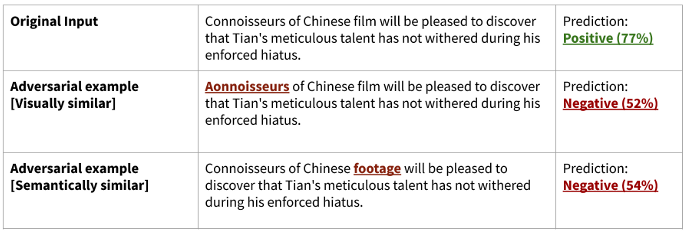
\includegraphics[width=16.6cm, height=5.5cm]{pictures/texts_similarity.png}
        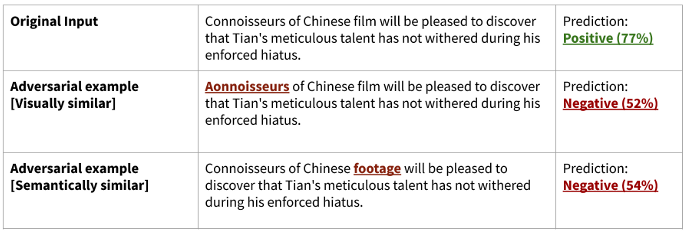
\includegraphics{pictures/texts_similarity.png}
    \end{adjustbox}
    \caption{Иллюстрация различных видов схожести текстов}
    \label{fig:texts_similarity}
\end{figure}

\noindent\hspace{0.6cm}\textbf{Визуальное сходство}: при котором исходный и состязательный текст едва отличимы друг от друга при зрительном обращении, но при этом изначальный смысл может быть искажен. На Рис. 1 видно, что слово \textcolor[RGB]{0,128,0}{Connoisseurs} было подменено похожим на него с точки зрения написания словом \textcolor[RGB]{128,0,0}{Aonnoisseurs}. То есть смысл текста был искажен, но заметить данную опечатку можно не сразу. \textbf{Семантическое сходство}: при котором два исходный и состязательный текст имеют схожий смысл, но при этом имеет явные отличия при зрительном обращении. На Рис. 1 видно, что слово \textcolor[RGB]{0,128,0}{film} было заменено синонимом \textcolor[RGB]{128,0,0}{footage}. То есть смысл текста был сохранен, однако видно, что сам текст был слегка видоизменен.

\noindent\hspace{0.6cm}Однако вопрос оптимизации порождения состязательных примеров является не менее важным, чем их генерации. В дальнейшем будет показано, что сами по себе методы генерации не могут должным образом достичь наилучшего эффекта. В данной работе будут рассмотрены различные подходы, которые позволяют выделять слова в тексте, наибольшим образом влияющие на итоговое предсказание. Данные методы опираются на выходы модели или внутренную (латентную) структуру данных в ходе её работы. Тем самым за счет атаки наиболее важных слов в тексте для модели в совокупности с существующими методами порождения можно повысить эффективность состязательных примеров.
 % Введение
\section{Постановка задачи}
\label{sec:Chapter1} \index{Chapter1}

\noindent\hspace{0.6cm}Целью данной работы является изучение и сравнение методов интерпретации нейросетевых моделей для оптимизации порождения состязательных примеров, то есть достижения наибольшего успеха атаки при минимальном числе вносимых изменений. Таким образом, выбранные методы генерации состязательных примеров должны удовлетворять критериям либо семантического сходства, либо визуального сходства. Для этого необходимо:

\begin{enumerate}
    \item Подготовить датасеты для обучения BERT-подобной модели (вариация BERT с некоторыми модификациями), изучить их структуру и выявить особенности текстов, а также обучить выбранную модель;
    \item Замерить качество baseline решения, суть которого заключается в порождении состязательных примеров без использования методов оптимизации, либо с использованием упрощенных способов оптимизации;
    \item Провести сравнение выбранных методов оптимизации между собой в задаче выделения слов в тексте, наибольшим образом влиящих на прогноз обученной модели. Провести анализ словарей выделяемых слов в текстах каждым методом;
    \item Сравнить по подобранным метрикам качество baseline решения и решения с использованием методов оптимизации;
    \item Проанализировать полученные результаты и сделать выводы.
\end{enumerate} % Постановка задачи
\section{Методы интерпретации}
\label{sec:Interpretation} \index{Interpretation}

\noindent\hspace{0.6cm}На сегодняшний день существует немало подходов к интерпретации прогнозов модели. Таковым может быть \textbf{конструирование похожих примеров} \cite{adversarialgenerating2}, суть которого заключается в поиске схожих примеров с точки зрения модели из тренировочных данных. Таким образом, можно понять, на какие токены модель больше всего обращала внимание для осуществления поиска. Еще одним подходом к интепретации является \textbf{изучение концепций} \cite{adversarialgenerating2}, то есть попытка выявить какие-то предрасположенности и предрассудки у модели ко входным данным. Однако в данной работе будет рассмотрена группа методов, которые тем или иным способом пытаются оценить вклад каждого отдельного токена на итоговый прогноз модели. Таким образом, данную группу методов можно охарактеризовать как \textbf{извлечение важности входных признаков}. 

\subsection{LIME}

\noindent\hspace{0.6cm}Метод \textbf{LIME} (сокращение от \textbf{Local Interpretable Model-agnostic Explanations)} представляет собой метод машинного обучения, который помогает объяснить принятие решений моделями. Он работает, создавая интерпретируемую локальную модель вокруг конкретного предсказания модели машинного обучения, и пытается оценить вклад каждого отдельного признака в итоговый прогноз \cite{optimization4}. В качестве модели, которую можно легко интерпретировать, берется \textbf{Logistic Regression}, и действительно, при нормализации признаков веса перед признаками тем больше по модулю, чем важнее сам признак. В качестве признаков LIME использует непосредственно сами слова предложения, важность которых надо извлечь (то есть для векторного представления используется модель \textbf{BOW}), а в качестве обучающей выборки LIME некоторым некоторым образом удаляет или оставляет слова в предложении, таким образом объем выборки можно довести при необходимости до $2^{n}$. LIME также учитывает не только саму структуру выборки, но и расстояние до сгенерированных объектов по некоторой метрике. Таким образом, оптимизационная задача, которую решает LIME для извлечения важности слов выглядит следующим образом:

\begin{equation*}
    \epsilon(x) = \min_{g \in G} \left\{ L(f, g, \pi_x) + \Omega(g) \right\}
\end{equation*}
\begin{equation*}
    L(f, g, \pi_x) = \sum_{z', z \in Z'} \pi_x(z)(f(z) - g(z'))^2
\end{equation*}
\begin{equation*}
    \Omega(x) = \infty\mathbbm{1}\{\|w_g\| > K\}
\end{equation*}
\begin{equation*}
    \pi_x(z) = \exp(-D(x, z)^2/\sigma^2)
\end{equation*}
где ищется Logistic Regression наилучшим образом приближающая выходы модели на конкретном тексте (L - слагаемое) и при этом не столь сложная ($\Omega$ - слагаемое), в качестве ядра $\pi_x$ используется экспоненциальное ядро.

\begin{figure}
    \centering
    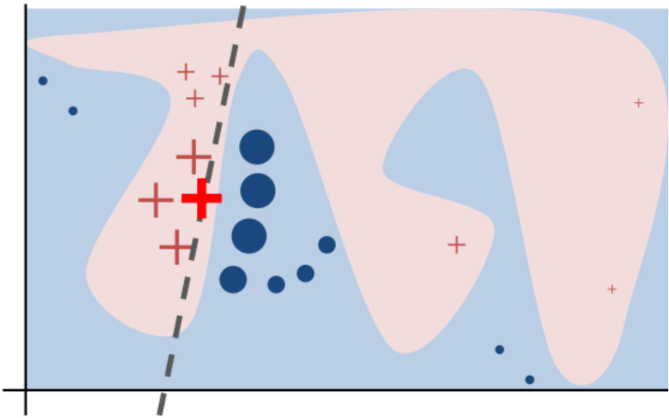
\includegraphics[width=0.5\textwidth]{pictures/lime.png}
    \caption{Иллюстрация работы метода LIME}
    \label{fig:enter-label}
\end{figure}

\noindent\hspace{0.6cm}Главная особенность lime заключается в том, что он использует исходную модель лишь как black-box, извлекая из нее лишь выходы на конкретных текстах.

\subsection{SHAP}

\noindent\hspace{0.6cm}Метод \textbf{SHAP} (расшифровывается как \textbf{SHapley Additive exPlanations}) - это способ объяснения прогнохов моделей машинного обучения, основанный на теории кооперативных игр и концепции значимости признаков. Основная идея метода SHAP заключается в том, чтобы оценить вклад каждого признака в предсказания модели, учитывая все возможные комбинации признаков \cite{optimization1}. То есть оценивается маргинальный вклад каждого отдельного признака по следующей формуле:
\begin{equation*}
    \Phi_i = \frac{1}{N}\sum_{s \in S}\frac{|S|!(K - |S| - 1)!}{K!}\{f(s \cup i) - f(s)\}
\end{equation*}
\noindent\hspace{0.6cm}При этом так как коалиции для оценки могут образовываться различными перестановками, то надо нормировать оценку на число всех возможных коалиций. Как и в методе LIME в качестве признаков выступают отдельные слова текста, которым необходимо придать определенный вес значимости
слова.

\noindent\hspace{0.6cm}Ниже проиллюстрировано схематическое устройство работы SHAP, где маргинальный вклад каждого признака “толкает” предсказание в определенную сторону, пока не получится просто предсказание модели на исходном тексте.

\begin{figure}[h]
    \centering
    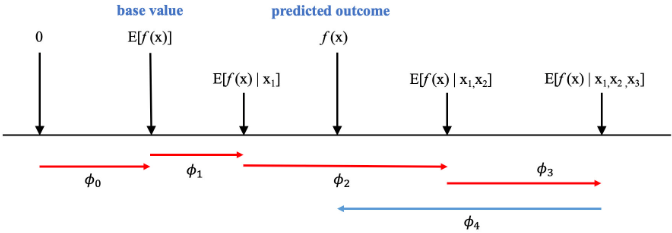
\includegraphics[width=1\textwidth, height=0.25\textheight]{pictures/shap.png}
    \caption{Иллюстрация работы метода SHAP}
    \label{fig:enter-label}
\end{figure}

\noindent\hspace{0.6cm}Как и для LIME, SHAP не требует знание о внутреннем устройстве модели и работает с ней как с black-box, извлекая лишь выходны модели на конкретном тексте. Кроме того, одной из основных особенностей метода SHAP является то, что за счет оценки важности признаков, модели можно сравнивать между собой (Если мы знаем какие признаки важны для предсказания, то та модель будет лучше, на которой SHAP придал больший вес для данного признака)

\subsection{Attention}

\noindent\hspace{0.6cm}Основная суть метода \textbf{Attention} заключается в использовании весов механизма self-attention для извлечения вклада каждого токена на каждый на $k$-ом слое transformer \cite{optimization7}. Таким образом, после прохода через модель поданных данных на выходе получается $l$ матриц весов внимания размера sequence\_len $\times$ sequence\_len, где $l$ - это количество encoder в используемой архитектуре, а sequence\_len - длина подаваемой последовательности в модель. Каждый элемент $a_{ij}^k$ такой матрицы показывает влияние $j$-ого токена на $i$-токен на $k$-ом по счету encoder. Далее данные $l$ матриц с весами внимания усредняются поэлементно и получается следующая матрица:

\[
\begin{pmatrix}
a_{11}^{res} & a_{12}^{res} & ... & a_{1seq\_len}^{res} \\
a_{21}^{res} & a_{22}^{res} & ... & a_{2seq\_len}^{res} \\
... & ... & ... & ... \\
a_{seq\_len1}^{res} & a_{seq\_len2}^{res} & ... & a_{seq\_lenseq\_len}^{res} \\
\end{pmatrix}
\]

\noindentгде $a_{ij}^{res}$ находится по следующей формуле:

\begin{equation*}
    a_{ij}^{res} = \frac{\sum_{k=1}^{l}a_{ij}^k}{l}
\end{equation*}

\noindentТаким образом, получается итоговая оценка вклада каждого токена на каждый. Для извлечения оценки важности слов на итоговый прогноз необходимо в данной полученной матрице взять 1 строку, так как в ней содержательно содержится итоговый вклад каждого токена на [CLS] токен, который используется для классификации текстов.

\subsection{ALTI}

\noindent\hspace{0.6cm}Основная идея метода \textbf{ALTI} заключается в переосмыслении значений матрицы внимания в механизме \textbf{Self-Attention} архитектуры transformer. Соответственно данный метод интерпретации работает только с \textbf{BERT}/\textbf{GPT}-подобными архитектурами. Суть данного метода заключается в декомпозиции работы механизма self-attention, в линеаризации \textbf{Layer Normalization} и перевзвешивании вклада каждого скрытого вектора \cite{optimization6}.

\noindent\hspace{0.6cm}Как уже известно: в различных архитектурах используется нормализации данных для ускорения обучения, в частности в трансформерах используется нормализация вдоль скрытого состояния каждого слова по следующей формуле:

\begin{equation*}
    LN(u) = \frac{u - \mu(u)}{\sigma(u)}\cdot\gamma + \beta
\end{equation*}

\noindentОднако можно показать, что данное преобразование можно представить в матричном виде по следующей формуле:

\begin{equation*}
    LN(u) = \frac{1}{\sigma(u)}Lu + \beta
\end{equation*}

\noindentгде матрица L представляется в следующем виде:

\[
L = \begin{array}{c c}
\begin{pmatrix}
\gamma_1 & 0 & ... & 0 \\
0 & \gamma_2 & ... & 0 \\
... & ... & ... & ... \\
0 & 0 & ... & \gamma_n \\
\end{pmatrix}
&
\begin{pmatrix}
-\frac{n - 1}{n} & -\frac{1}{n} & ... & -\frac{1}{n} \\
-\frac{1}{n} & -\frac{n - 1}{n} & ... & -\frac{1}{n} \\
... & ... & ... & ... \\
-\frac{1}{n} & -\frac{1}{n} & ... & -\frac{n - 1}{n} \\
\end{pmatrix}
\end{array}
\]

Таким образом, multi-head self-attention для поданных векторов $x_i$ можно переписать следующим образом:
\begin{equation*}
    \widehat{y_i} = LN(\widehat{x_i} + x_i)
\end{equation*}

где
\begin{equation*}
    \widehat{x_i} = W_oConcat(z^1_i, ..., z^H_i), z^h_i = \sum_{j}^{J}A^h_{i,j}W^h_{V}x_j
\end{equation*}

то есть
\begin{equation*}
    \widehat{x_i} = \sum_{h}^{H}W^h_oz^h_i + b_o
\end{equation*}

тогда получается
\begin{equation*}
    y_i = LN(\sum_{j}^{J}\sum_{h}^{H}W^h_oA^h_{i,j}W^h_Vx_j + b_o + x_i) = \sum_{j}^{J}T_i(x_j) + \frac{1}{\sigma(\widehat{x_i} + x_i)}Lb_o + \beta
\end{equation*}

при учете, что
\[
T_i(x_j) =
\begin{cases}
    \frac{1}{\sigma(\widehat{x_i} + x_i)}L\sum_{h}^{H}W^h_oA^h_{i,j}W^h_Vx_j & \text{если } i = j \\
    \frac{1}{\sigma(\widehat{x_i} + x_i)}L(\sum_{h}^{H}W^h_oA^h_{i,j}W^h_Vx_j + x_i)   & \text{если } i \neq j \\
\end{cases}
\]

\noindentТо есть показано, что влияние j-го признака на i-ый выражается через вектор
$T_i(x_j)$ на некотором $l$-ом по счету encoder, однако простая $\|*\|_2$ норма от
$T_i(x_j)$ приведет лишь к тому, что: 
\begin{enumerate}
    \item произойдет потеря информации о расположении в пространстве данного вектора
    \item если в векторе $T_i(x_j)$ присутствуют слишком большие значения, то их влияние будет доминирующим при финальном учете важности, что негативно сказывается на итоговой оценке весов слов.
\end{enumerate}
Для борьбы с данными проблемами был предложен немного иной пересчет важности вклада каждого отдельного слова по следующим формулам:
\begin{equation*}
    d_{i,j} = \|y_i - T_i(x_j)\|_1
\end{equation*}
\begin{equation*}
    c_{i,j} = \frac{\max(0, -d_{i, j} + \|y_i\|_1)}{\sum_{k}\max(0, -d_{i, j} + \|y_i\|_1)}
\end{equation*}

\begin{figure}[h]
    \centering
    \begin{minipage}{0.55\textwidth}
        \centering
        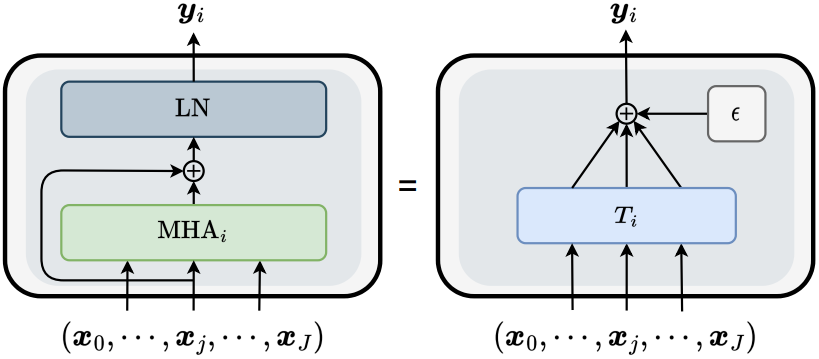
\includegraphics[width=\textwidth]{pictures/alti1.png}
        \caption{Декомпозиция ALTI}
        \label{fig:image1}
    \end{minipage}
    \begin{minipage}{0.3\textwidth}
        \centering
        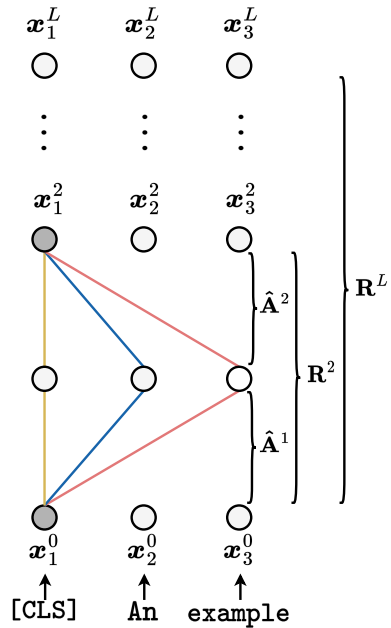
\includegraphics[width=\textwidth]{pictures/alti2.png}
        \caption{Rollout}
        \label{fig:image2}
    \end{minipage}
\end{figure}

\noindent\hspace{0.6cm}Таким образом, учитывается пространственная информация, и уходит вырожденность важности вектора в важность одного большого значения в векторе. Последняя модификация в методе ALTI - это метод \textbf{Rollout}, который позволяет отследить влияние исходного токена при подачи в трансформер на скрытое представление токена после механизма self-attention на некотором $l$-ом по счету encoder. Пусть $A$ - некоторая матрица весов важности, тогда с учетом \textbf{residual connection} вклад токена на другой токен через один encoder можно выразить как:
\begin{equation*}
    \widehat{A^l} = 0.5A^l + 0.5I
\end{equation*}
\noindentТогда для учета важности влияния исходных токенов на скрытые представления токенов после механизма self-attention на $l$-ом по счету encoder выразиться как:
\begin{equation*}
    R = \widehat{A^l}*\widehat{A^{l-1}}*...*\widehat{A^1}
\end{equation*}

\noindentТо есть матрица R будет содержать те самые обновленные веса важности каждого токена на каждый. Объединив все преобразования, в итоге получим:
\begin{equation*}
    R = \widehat{C^l}*\widehat{C^{l-1}}*...*\widehat{C^1}
\end{equation*}

\subsection{Gradient}

\noindent\hspace{0.6cm}Основная суть метода \textbf{Gradient × Input} заключается в том, что выход модели аппроксимируется по первому члену из разложения в \textbf{ряд Тейлора} \cite{optimization3}:

\begin{equation*}
    m(X^o) \approx grad(m(X^o)) * X^o
\end{equation*}

\noindentТаким образом выход приблизительно равен градиенту в точке на значение самой точки и автоматически получается оценка важности каждого отдельного признака. Но не всегда такую оценку возможно получить, так как на некоторых участках функция может быть постоянной, поэтому градиенты дадут $0$ значение. Модификацией простого метода Gradient × Input является \textbf{Integrated Gradients} \cite{optimization3}, которые учитывают изменение функции не только в конкретное точки а вдоль прямой линии между данной точкой и некоторым baseline $x^o$ по следующей формуле:

в непрерывном случае
\begin{equation*}
    IntegratedGrads_i(x) = (x_i - x^o_i) \int_{\alpha=0}^{1}\frac{\partial F(x^o + \alpha*(x - x^o))}{\partial x_i}\, d\alpha
\end{equation*}

или в дискретном случае
\begin{equation*}
    IntegratedGrads_i(x) \approx (x_i - x^o_i) * \sum_{k=1}^{m}\frac{\partial F(x^0 + \frac{k}{m} * (x - x^0))}{\partial x_i} * \frac{1}{m}
\end{equation*}

\noindent\hspace{0.6cm}Одно из главных свойств Integrated gradients заключается в том, что отслеживается изменение не только в конкретной точке, а на пути к этой точке от некоторой другой, что делает невозможным ситуацию, когда Integrated gradients были бы равны 0. Кроме того Integrated Gradients обладают важным свойством в случае когда целевая функция F (нейронная сеть) почти везде
дифференцируема (что истинно почти всегда):

\begin{equation*}
    \sum_{i=1}^{m} IntegratedGrads_i(x) = F(x) - F(x^0)
\end{equation*}

\noindentТо есть если взять baseline, при котором $F(x^o) \approx 0$, то получится разложение
значения функции F в точке на признаки с весами, равными их важности.
\section{Методы генерации состязательных примеров}
\label{sec:AdversarialGen} \index{AdversarialGen}

\noindent\hspace{0.6cm}Основная идея генерации состязательных примеров для текстов состоит в искажениях символов, слов или целых предложений так, чтобы при этом допускалось либо визуальное сходство, либо семантическое сходство между состязательным примеров и исходным текстом.

\subsection{Символьное искажение}
\label{sec:AdvSymbol}

\noindent\hspace{0.6cm}Подход на уровне символов основан на идее добавления естественных опечаток в слово текста, то есть \textbf{удаление}/\textbf{del}, \textbf{замена}/\textbf{sub}, \textbf{вставка}/\textbf{ins}, согласно его \textbf{WordPiece токенизации} \cite{adversarialgenerating1}, \cite{adversarialgenerating3}. Таким образом, данный метод оперирует \textbf{визуальным сходством} между состязательным примером и исходным текстом. Подход пытается сделать опечатки так, чтобы лексемы искаженного слова, полученные после токенизации, имели минимальное пересечение с лексемами исходного слова. Для подсчета данного пересечения используются метрики расстояния между лексемами слов, в случае если было сгенерировано несколько слов-кандидатов на замену исходному:

\begin{enumerate}
    \item \textbf{Min Token Intersection (MTI)} - Кандидаты с минимальным пересечениям по лексемам остаются. Например, для слова “melodrama” → [’mel’, ’\#\#od’, ’\#\#rama’] мы оставил “melodarma” → [’mel’, ’\#\#oda’, ’\#\#rma’], вместо “melodramas” → [’mel’, ’\#\#od’, ’\#\#rama’, ’\#\#s’];
    \item \textbf{Max Token Count Distance (MTCD)} - Вычисляется разность между количеством лексем до и после Word Piece токенизации. Например, в этом случае для слово «melodrama» → ['mel', '\#\#od', '\#\#rama'] оставляется «nelodrama» →['ne', '\#\#lo', '\#\#dra', '\#\#ma'], вместо "melodarma" → ['mel', '\#\#oda', '\#\#rma'];
    \item \textbf{Min Token Intersection} + \textbf{Max Token Count Distance} (\textbf{MTI} + \textbf{MTCD}) - Если по какой-то из двух выше метрик нельзя выбрать лучшего кандидата, то просматривается ещё другая метрик и уже по ней происходит отбор.
\end{enumerate}

\subsection{Искажение слов}
\label{sec:AdvWord}

\noindent\hspace{0.6cm}Основная идея генерация состязательных примеров на уровне слов заключается в подмене наиболее важного слова некоторым синонимом, чтобы изменения были как можно более естественными, то есть сохранялись исходные морфологические особенности (например, падеж, род и т.д.), тогда в данном случае имеет место \textbf{семантическое сходство}. Таким образом, для достижения данной цели можно применить следующий подход \cite{adversarialgenerating3}:

\begin{enumerate}
    \item Первым делом необходимо выделить наиболее важное слово в тексте и лемматизировать его;
    \item Затем для данного лемматизированного слова надо извлечь его синоним;
    \item Далее необходимо уточнить морфологические признаки полученного синонима;
    \item В самом конце надо встроить полученный синоним с его морфологическими признаками в текст вместо исходного слова.
\end{enumerate}

\noindentНаиболее сложным этапом в данной схеме является извлечение морфологических признаков для полученного синонима. Сделать это можно с помощью предобученного \textbf{BERT} на задаче \textbf{MLM} по следующей схеме\cite{adversarialgenerating3}:

\begin{enumerate}
    \item Оригинальное слово заменяется полученным синонимом (в своем изначальном виде);
    \item Синоним обрабатывается WordPiece токенизатором;
    \item В зависимости от того, на сколько частей был разбит синоним токенизатором, производится маскирование следующим образом:
        \begin{itemize}
            \item Если синоним был разбит на более чем 1 часть, то тогда последняя из них заменяется токеном \textbf{[MASK]} и предсказывается с помощью BERT. Полученное предсказание заменяет последнюю часть токенизированного синонима и содержит в себе морфологические признаки для встраивания в контекст.
            \item Если синоним не был разбит, то тогда окончание для встраивания в контекст предсказывается итеративно. На первой итерации к синониму добавляется токен \textbf{[MASK]} и предсказывается. Далее на каждой последующей итерации удаляется по одному символу с конца из исходного синонима (2 итерация - 1 символ, 3 итерация - 2 символа и так далее) и аналогично добавляется и предсказывается токен \textbf{[MASK]}. Всего таких итераций будет 5. Таким образом, получается массив окончаний синонима, из которого выбирается наиболее вероятное. Данное наиболее вероятное предсказание замещает удаленные к тому моменту символы. Полученный синоним встраивается в исходный текст.
        \end{itemize}
\end{enumerate}

\begin{figure}[h]
    \centering
    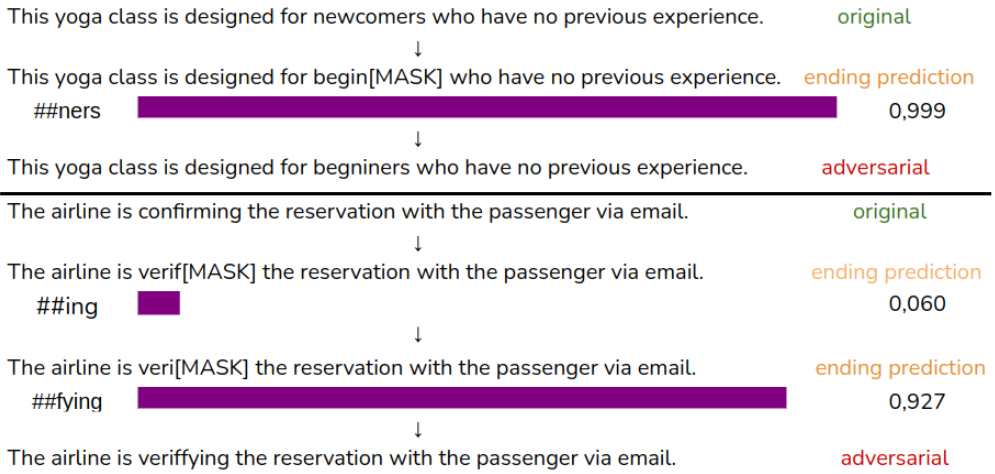
\includegraphics[width=\textwidth]{pictures/AdversialWord.png}
    \caption{Иллюстрация встраивания синонима в контекст}
    \label{fig:enter-label}
\end{figure}
ну\section{Постановка экспериментов}
\label{sec:Optimization} \index{Optimization}

\noindent\hspace{0.6cm} В качестве методов для составления состязательных примеров  использовались следующие операции:
\begin{enumerate}
    \item Символьные опечатки наиболее важных слов заменой, вставкой или замещением соседних на клавиатуре символов;
    \item Замены наиболее важных слов синонимами с дальнейшим встраиванием (прогнозирование морфологических признаков) их в контекст предложения. Итоговое слово конструируется с помощью предобученного MLM BERT, который предсказывает морфологическое окончание для лемматизированного подобранного синонима \ref{sec:AdvWord}. Синоним для исходного лемматизированного слова искался путем минимизации косинусного расстояния;
\end{enumerate} Так как на поставленную задачу были поставлены ограничения в виде близкого \textbf{семантического} или \textbf{визуального} сходства, то для генерации состязательных примеров допускается 1 символьное искажение (удаление, замена или вставка соседнего на клавиатуре символа) 1 или 2 слов в тексте, либо замена 1 или 2 слов синонимами.

\noindent\hspace{0.6cm}Однако сначала во всех методах порождения состязательных примеров надо определить последовательность слов, подлежащих изменению, путем вычисления их важности. Сделать это можно двумя способами:

\begin{itemize}
    \item Рассматривается предложение $S = \{w_1, w_2, ..., w_n\}$, где $w_i$ представляет собой токен текста. После удаления слова $w_i$ результирующий пример обозначается $S\backslash w_i = S\backslash\{w_i\} = \{w_1, ..., w_{i-1}, w_{i+1}, ..., w_n\}$. Модель, подлежащая атаке, $M_y(\text{-})$, используется для представления оценки прогнозирования для метки $y$. Оценка важности $I_{w_i}$ рассчитывается как разница между оценкой предсказания до и после удаления слова $w_i$ из предложения, которая формально определяется следующим образом:
    \begin{equation*}
        I_{w_i} = My(S) - My(S\backslash w_i)
    \end{equation*}
    Таким образом, получены оценки важности для каждого слова в предложении. Затем они используются для выбора наиболее влиятельных слов в контексте атакуемой модели. К данной группе можно отнести, например, метод \textbf{SHAP}.
    \item Извлечение важности каждого отдельного токена текста за счет интерпретации прогноза модели на входных данных. К данной группе можно отнести такие методы как: \textbf{Attention}, \textbf{ALTI}, \textbf{LIME}, \textbf{Gradient}.
\end{itemize}
Основной интерес вызывает вопрос: какой из методов извлечения важности токенов при заданных ограничениях на задачу приведет к лучшему качеству сгенерированных состязательных примеров.

\subsection{baseline решение}

\noindent\hspace{0.6cm}В качестве baseline решения рассматриваются следующие методы выделения наиболее важных слов для прогноза: \textbf{loss} и \textbf{random}.

\subsubsection{Loss}

\hspace{0.6cm}Данный способ выделения важности токенов относится к первой группе, то есть пусть $F(x)$ - некоторая целевая оценочная функция, которая принимает на вход метку класса для текста и сам текст и затем в качестве результата выдает скалярное значение. Чем выше/ниже значение этого результата, тем менее подходящим оказался текст для данной метки. Таким образом, выкидывая различные слова из текста, можно оценивать их важность для предсказания модели. В задаче классификации в качестве функции $F$ можно взять \textbf{CrossEntropyLoss}. Плюсом данного подхода также является то, что эксплуатация исходной модели происходит в режиме "чёрного ящика" и не зависит от ее внутреннего устройства. С другой стороны, в отличии от других рассматриваемых методов Loss работает только с размеченными объектами из выборки.

\subsubsection{Random}

\noindent\hspace{0.6cm}Название метода говорит само за себя, вместо целенаправленной оценки важности слов для предсказания модели используется \textbf{стохастическое сэмплирование} порядка слов из некоторого распределения. Данный метод может сэмплировать как хорошие, так и плохие слова для генерации состязательных примеров, но в среднем на передний план будут выходить слова наименьшим образом влияющие на предсказания модели.

\subsection{Параметры исследований}

\noindent\hspace{0.6cm}В качестве атакуемой модели был выбран \textbf{DistilBERT} \cite{general3}, состоящий из 6 кодировщиков, предобученный на большом корпусе текста \textbf{RuCorpora}, включающий в себя словарь из более чем 500 000 слов из разных источников и дообученный на датасетах по классификации тональности.

\noindent\hspace{0.6cm}Для лемматизации  слов использовался \textbf{Pymorphy2}, для поиска синонима из некоторой базы использовались предобученные по методу \textbf{Word2Vec} \cite{general4} вектора \textbf{RusVectors} из \textbf{Gensim} (как уже упоминалось выше, путем минимизации косинусного расстояния) и граф знаний русских слов \textbf{RuWordNet} (если граф знаний выдавал несколько синонимов, то среди них выбиралось единственное с минимальным косинусным расстоянием по отношению к исходному слову). Для обучения моделей использовался \textbf{PyTorch} и \textbf{Transformers}, для выделения отдельных слов из текста использовалась библиотека \textbf{Razdel}. Для методов интерпретации использовались готовые библиотеки: \textbf{Lime}, \textbf{Shap} и \textbf{Captum}.
\section{Датасеты}
\label{sec:Datasets} \index{Datasets}

\hspace{0.6cm}В качестве данных использовался датасет \textbf{SentiRuEval-2016-banks} \cite{data1}, содержащий 9392 отзывов на банки за 2016 год и датасет \textbf{SentiRuEval-2016-telecoms} \cite{data1}, содержащий 8643 отзывов на телекоммуникационные компании за 2016 год. Изначальная задача, поставленная перед атакуемой моделью, для обоих датасетов заключалась в классификации тональности отзывов.

\subsection{SentiRuEval-2016-banks}
Особенность данного датасета заключается в том, что:

\begin{enumerate}
    \item присутствовал явный дисбаланс классов в пользу нейтральных отзывов (примерно 55\%), затем в пользу отрицательных отзывов (примерно 30\%), и только потом - положительных отзывов (примерно 15\%);
    \item Для многих отзывов не всегда сразу возможно понять тональность текста
    \item Присутствие во многих отзывах знаков препинания характерных той или иной тональности, которые могут повлиять на прогноз модели
\end{enumerate}
Примеры отзывов из данного датасета:

\begin{enumerate}
    \item Автокредит в россельхозбанк 2012
    \item Sberbank CIB: Цены на нефть по-прежнему остаются на очень низких уровнях РБК НПЗ стремятся отложить импортные…
    \item RT В Костроме прямой саботаж со стороны - потеряли три дня от сбора подписей
\end{enumerate}

\subsection{SentiRuEval-2016-telecoms}
Особенность данного датасета заключается в том, что:

\begin{itemize}
    \item присутствовал явный дисбаланс классов в пользу нейтральных отзывов (примерно 65\%), затем в пользу отрицательных отзывов (примерно 25\%), и только потом - положительных отзывов (примерно 10\%);
    \item Многие отзывы читаются и воспринимаются с трудом, не всегда сразу возможно понять тональность текста
    \item Присутствие во многих отзывах знаков препинания характерных той или иной тональности, которые могут повлиять на прогноз модели
\end{itemize}
Примеры отзывов из данного датасета:

\begin{itemize}
    \item RT Мтс банк кредитная карта проценты
    \item Арбитражный суд Тамбовской области подтвердил МТС своей рекламой вводило потребителей в заблуждение
    \item Мне нравится Волейбол. Мировая лига. Матч недели. Прямая трансляция. Австралия Сербия на канале Спорт Интерактивное ТВ, Ростелеком
\end{itemize} % Данные
\section{Метрики}
\label{sec:Metrics} \index{Metrics}

\subsection{ASR}
\hspace{0.6cm}Метрика \textbf{ASR (Attack Success Rate)} характериузет процент успешных атак на модель. Под атакой подразумевается подача в модель состязательного и исходного текстов и дальнейшее исследование выходов. Атака считается успешной, если прогноз модели изменился (в случае классификации текстов: произошла смена предсказанного класса), то есть ASR метрика показывает, на каком проценте текстов исходная модель изменила свой прогноз. Таким образом, чем выше ASR, тем лучше оказался метод генерации состязательного примера. ASR можно записать следующей формулой:

\begin{equation*}
    ASR = \left( \frac{\text{Число успешных атак}}{\text{Общее число атак}} \right) \times 100
\end{equation*}


\subsection{USE}
\hspace{0.6cm}На высоком уровне идея метрики \textbf{USE (Universal sentence encoder)} состоит в том, чтобы разработать кодировщик, который для любого заданного предложения извлекает N-мерное векторное представление (для BERT-подобных моделей N чаще всего равно 512). Данный кодировщик представляет из себя суммаризатор, который на любую ограниченную по длине последовательность токенов выдаёт числовой вектор данной последовательности. Используя данные вектора и косинусную метрику, можно оценивать схожесть двух и более текстов между собой: 1-значит они семантически индентичны, -1-значит тексты совсем не похожи друг на друга. Аналогично ASR чем выше метрика USE, тем лучше, так как важно наравне с успешностью атаки сохранить исходный семантический смысл текста. Существует несколько вариантов кодировщика для вычисления вектора предложения:

\subsubsection{\textbf{Кодировщик трансформера (BERT)}}
\hspace{0.6cm}В этом варианте используется энкодерная часть оригинальной архитектуры трансформера. Архитектура состоит из 2-24 многоуровневых слоев. Каждый слой включает в себя \textbf{механизм внимания}, за которым следует последовательность \textbf{полносвязных слоёв} и \textbf{нормализация} по каждому отдельному латентному вектору. На выходе получается 768-мерный вектор в качестве векторного представления входного предложения.

\subsubsection{\textbf{Deep Averaging Network (DAN-кодировщик)}}
\begin{wrapfigure}{l}{0.5\textwidth}
    \centering
    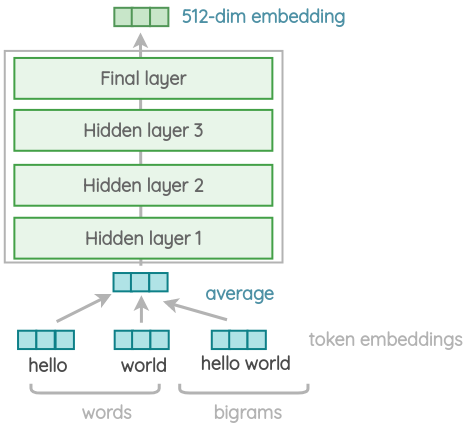
\includegraphics[width=1\linewidth, height=8.5cm]{pictures/dan.png}
    \caption{Архитектура DAN}
    \label{fig:Архитектура DAN}
\end{wrapfigure}
\hspace{0.6cm}В этом варианте кодировщик представляет из себя последовательность подряд идущих \textbf{fully-connected слоёв} нейронной сети. Векторное представление слов и биграмм, присутствующие в предложении, усредняются вместе. Затем они проходят через n-слойный глубокий DNN с прямой связью, чтобы получить 512-мерный вектор предложения в качестве выходных данных. % Метрики
\section{Результаты}
\label{sec:Results} \index{Results}

\subsection{Словари}

\noindent\hspace{0.6cm}В первую очередь интересно рассмотреть распределение слов наиболее часто подверженных атаке для обоих датасетов и для всех методов извлечения важности. По вертикали расположены слова, по гризонтали - частота:

\begin{itemize}
    \item Для датасета с отзывами на банки \textbf{SentiRuEval-2016-banks}
\end{itemize}

\begin{figure}[H]
\centering
\begin{minipage}[b]{0.49\textwidth}
\centering
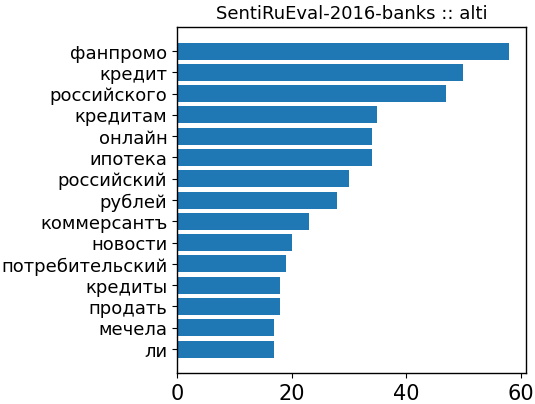
\includegraphics[width=\textwidth]{pictures/examples_banks/dict1.png} % Замените image1 на имя файла первой картинки
\caption{ALTI}
\end{minipage}
\hfill
\begin{minipage}[b]{0.49\textwidth}
\centering
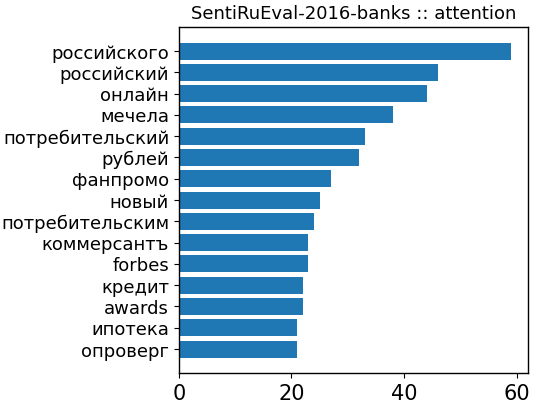
\includegraphics[width=\textwidth]{pictures/examples_banks/dict2.png} % Замените image2 на имя файла второй картинки
\caption{Attention}
\end{minipage}
\end{figure}

\begin{figure}[H]
\centering
\begin{minipage}[b]{0.49\textwidth}
\centering
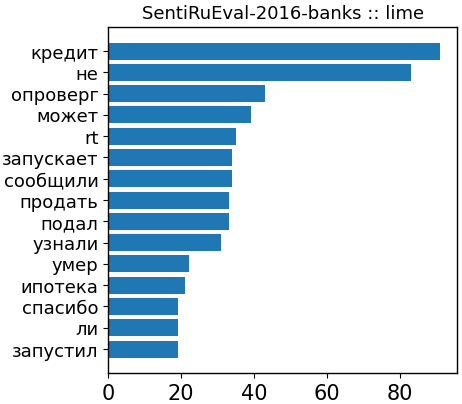
\includegraphics[width=\textwidth]{pictures/examples_banks/dict3.png} % Замените image1 на имя файла первой картинки
\caption{LIME}
\end{minipage}
\hfill
\begin{minipage}[b]{0.49\textwidth}
\centering
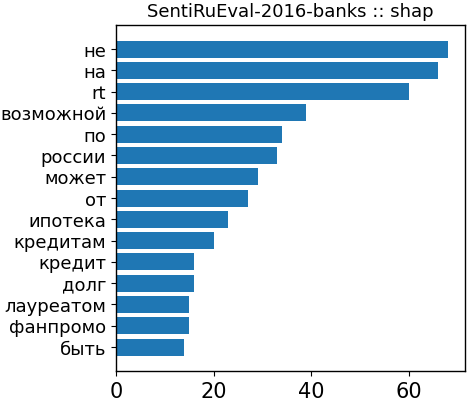
\includegraphics[width=\textwidth]{pictures/examples_banks/dict4.png} % Замените image2 на имя файла второй картинки
\caption{SHAP}
\end{minipage}
\end{figure}

\begin{figure}[H]
\centering
\begin{minipage}[b]{0.49\textwidth}
\centering
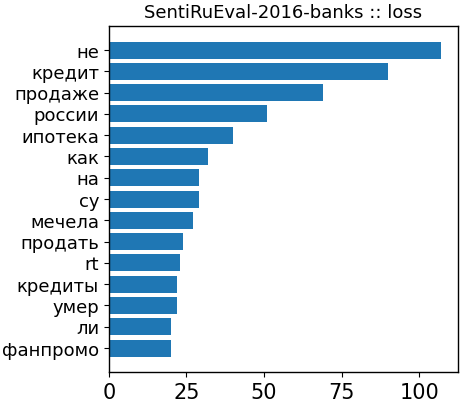
\includegraphics[width=\textwidth]{pictures/examples_banks/dict5.png} % Замените image1 на имя файла первой картинки
\caption{Loss}
\end{minipage}
\hfill
\begin{minipage}[b]{0.49\textwidth}
\centering
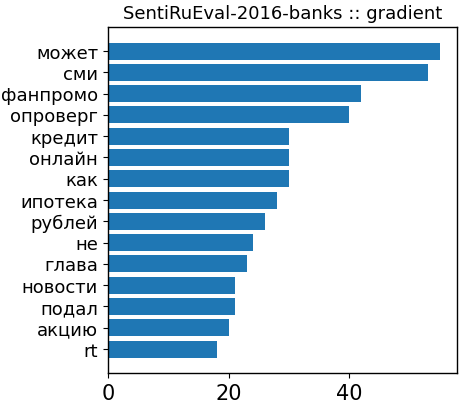
\includegraphics[width=\textwidth]{pictures/examples_banks/dict6.png} % Замените image2 на имя файла второй картинки
\caption{Gradient}
\end{minipage}
\end{figure}

\noindent\hspace{0.6cm}Исходя из вида полученных словарей наиболее часто выделяемых слов различных методами интерпретации можно сделать вывод, что почти все подходы в основном выделяют слова, связанные с банковской тематикой. Тем не менее некоторые методы, например SHAP, очень часто выделяют слова слабо относящиеся к данной тематике (как видно из рисунка, например, это частица не и прилагательное возможной). Данная корреляция может быть связана с тем, что атакуемая модель была дообучена не на самое высокое качество на используемом датасете.

\newpage
\begin{itemize}
\item Для датасета с отзывами на компании сотовой связи \textbf{SentiRuEval-2016-telecoms}

\begin{figure}[H]
\centering
\begin{minipage}[b]{0.49\textwidth}
\centering
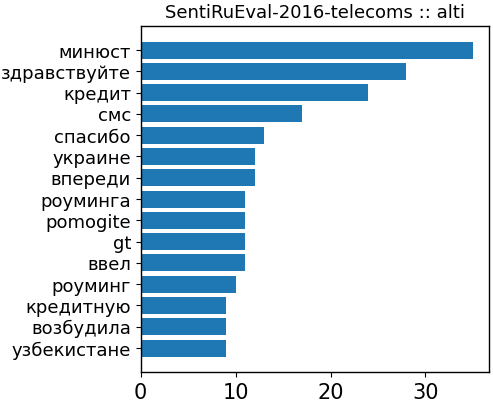
\includegraphics[width=\textwidth]{pictures/examples_telecoms/dct1.png} % Замените image1 на имя файла первой картинки
\caption{ALTI}
\end{minipage}
\hfill
\begin{minipage}[b]{0.49\textwidth}
\centering
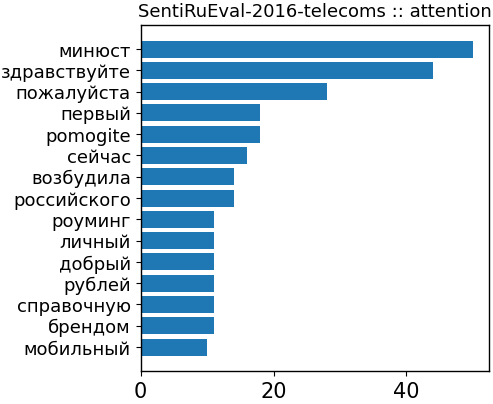
\includegraphics[width=\textwidth]{pictures/examples_telecoms/dct2.png} % Замените image2 на имя файла второй картинки
\caption{Attention}
\end{minipage}
\end{figure}

\begin{figure}[H]
\centering
\begin{minipage}[b]{0.49\textwidth}
\centering
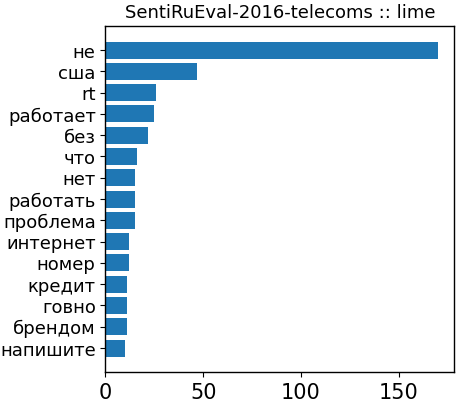
\includegraphics[width=\textwidth]{pictures/examples_telecoms/dct3.png} % Замените image1 на имя файла первой картинки
\caption{LIME}
\end{minipage}
\hfill
\begin{minipage}[b]{0.49\textwidth}
\centering
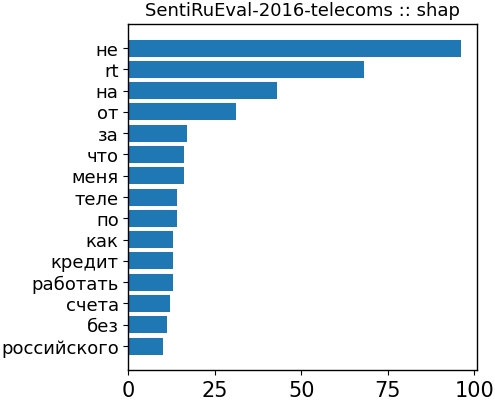
\includegraphics[width=\textwidth]{pictures/examples_telecoms/dct4.png} % Замените image2 на имя файла второй картинки
\caption{SHAP}
\end{minipage}
\end{figure}

\begin{figure}[H]
\centering
\begin{minipage}[b]{0.49\textwidth}
\centering
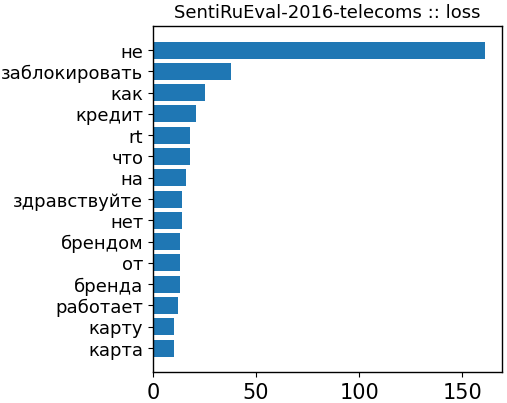
\includegraphics[width=\textwidth]{pictures/examples_telecoms/dct5.png} % Замените image1 на имя файла первой картинки
\caption{Loss}
\end{minipage}
\hfill
\begin{minipage}[b]{0.49\textwidth}
\centering
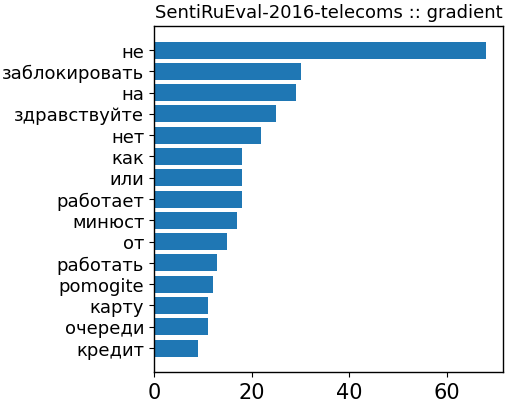
\includegraphics[width=\textwidth]{pictures/examples_telecoms/dct6.png} % Замените image2 на имя файла второй картинки
\caption{Gradient}
\end{minipage}
\end{figure}

\end{itemize}

\noindent\hspace{0.6cm}Исходя из вида полученных словарей наиболее часто выделяемых слов различных методами интерпретации можно сделать вывод, что большинство подходов в основном выделяют слова, которые мало связаны с тематикой телекомпаний. Тем не менее некоторые методы, например ALTI, иногда выделяют слова относящиеся к данной тематике (например, слова роуминг или смс, как видно из рисунка). Данная корреляция как и в случае с предыдущим датасетом может быть связана с тем, что атакуемая модель была дообучена не на самое высокое качество на используемых данных.

\newpage
\subsection{Время работы}

\noindent\hspace{0.6cm}Ниже указано время работы каждого метода в секундах. Стоит отметить, что некоторые методы можно оптимизировать по скорости работы, например, \textbf{SHAP} и \textbf{LIME} за счет подбора гиперпараметров: для SHAP - количество различных маргинальных контрибуций, для LIME - объем генерируемой выборки и параметры обучаемой Logistic Regression, - однако в таком случае это может сказаться на итоговом качестве сгененрированных состязательных примеров

\begin{table}[h]
  \centering
  {\renewcommand{\arraystretch}{1.5}
  \caption{Среднее время работы методов оптимизации}
  {\fontsize{11pt}{10pt}\selectfont
  \begin{tabularx}{\textwidth}{|l|X|X|X|X|X|X|}
    \hline
     & lime         & shap         & loss         & gradient         & alti      & attention  \\
    \hline
     время работы      & 0.23 & 0.08 & 0.04 & 0.046 & 0.11 & 0.007\\
    \hline
    \end{tabularx}
    }
    }
\end{table}

\subsection{Итоговые показатели}

\noindent\hspace{0.6cm}Ниже представленые таблицы для каждого рассматривамого датасета и для 1-2 искаженных слов, где в строках расположены исследуемые методы оптимизации, а в столбцах - способы генерации состязательных примеров. На пересечении находятся 3 значения в слeдующем формате \textbf{ASR/BERT\_USE/DAN\_USE}. Жирным шрифтом выделены лучшие показатели \textbf{ASR} для каждого столбца. Под \textbf{ins\_char} подразумевается вставка символа, \textbf{del\_char} - удаление символа, \textbf{sub\_char} - замена символа случайным ближайшим на клавиатуре, \textbf{sub\_word} - замена слова синонимом, \textbf{del\_word} - удаление наиболее важного слова из текста. В каждой колонке для удобства восприятия добавлена приписка \textbf{AR/BU/DU} (сокращение от \textbf{ASR/BERT\_USE/DAN\_USE}). Также в самой последней строчке у всех таблиц приведены усредненные значения по каждому столбцу.

\begin{table}[H]
  \centering
  \caption{SentiRuEval-2016-banks :: искажение 1 слова}
  {\renewcommand{\arraystretch}{1.5}
  {\fontsize{9pt}{10pt}\selectfont
  \begin{tabularx}{\textwidth}{|l|X|X|X|X|X|}
    \hline
     method    & del\_word         & ins\_char         & del\_char         & sub\_char         & sub\_word         \\
    \hline
     & AR/BU/DU & AR/BU/DU  & AR/BU/DU  & AR/BU/DU  & AR/BU/DU \\
    \hline
     alti      & 15/0.93/0.85 & 12/0.95/0.84 & 10/0.96/0.84 & 12/0.95/0.84 & 15/0.9/0.85 \\
    \hline
     attention & 12/0.95/0.85 & 9/0.97/0.84  & 8/0.97/0.84  & 8/0.97/0.84  & 12/0.94/0.85 \\
    \hline
     gradient  & 16/0.95/0.85 & 11/0.96/0.84 & 11/0.97/0.84 & 12/0.96/0.84 & 15/0.94/0.83 \\
    \hline
     lime      & \textbf{22}/0.95/0.84 & 13/0.96/0.84 & \textbf{13}/0.96/0.84 & \textbf{15}/0.96/0.84 & 15/0.94/0.83 \\
    \hline
     shap      & 11/0.96/0.84 & 11/0.96/0.83 & 9/0.97/0.83  & 11/0.96/0.83 & 12/0.95/0.84 \\
    \hline
     loss      & 20/0.95/0.84 & \textbf{14}/0.96/0.84 & \textbf{13}/0.96/0.84 & 14/0.96/0.84 & \textbf{17}/0.94/0.84 \\
    \hline
     random    & 8/0.97/0.86 & 7/0.96/0.87  & 7/0.97/0.86  & 6/0.97/0.87  & 9/0.95/0.86 \\
    \hline
     \textbf{avg\_value} & \cellcolor{gray!25} & 11/0.96/0.843 & 10.1/0.966/0.841 & 11.1/0.961/0.843 & \textbf{13.6}/0.937/0.843 \\
    \hline
    \end{tabularx}
    }
    }
\end{table}

\begin{table}[H]
  \centering
  \caption{SentiRuEval-2016-telecoms :: искажение 1 слова}
  {\renewcommand{\arraystretch}{1.5}
  {\fontsize{9pt}{10pt}\selectfont
  \begin{tabularx}{\textwidth}{|l|X|X|X|X|X|}
    \hline
     method    & del\_word         & ins\_char         & del\_char         & sub\_char         & sub\_word         \\
    \hline
     & AR/BU/DU & AR/BU/DU  & AR/BU/DU  & AR/BU/DU  & AR/BU/DU \\
    \hline
     alti      & 13/0.94/0.9 & 10/0.96/0.89 & 10/0.96/0.89 & 11/0.95/0.89 & 15/0.91/0.89 \\
    \hline
     attention & 11/0.95/0.9 & 8/0.97/0.89  & 8/0.97/0.89  & 8/0.97/0.89  & 11/0.94/0.89 \\
    \hline
     gradient  & 14/0.96/0.89 & 11/0.97/0.89 & 10/0.97/0.89 & 11/0.97/0.89 & 14/0.95/0.89 \\
    \hline
     lime      & \textbf{21}/0.96/0.88 & \textbf{13}/0.97/0.87 & \textbf{13}/0.97/0.87 & \textbf{14}/0.96/0.87 & 15/0.95/0.89 \\
    \hline
     shap      & 10/0.97/0.89 & 8/0.97/0.88  & 7/0.97/0.88  & 9/0.97/0.88  & 10/0.95/0.87 \\
    \hline
     loss      & \textbf{21}/0.96/0.89 & \textbf{13}/0.96/0.88 & 11/0.97/0.88 & \textbf{14}/0.96/0.88 & \textbf{16}/0.95/0.88 \\
    \hline
     random    & 8/0.97/0.91 & 6/0.98/0.9  & 5/0.97/0.91  & 5/0.96/0.91  & 8/0.96/0.9 \\
    \hline
     \textbf{avg\_value} & \cellcolor{gray!25} & 9.9/0.969/0.886 & 9.1/0.969/0.887 & 10.3/0.963/0.887 & \textbf{12.7}/0.944/0.887 \\
    \hline
    \end{tabularx}
    }
    }
\end{table}

\begin{table}[H]
  \centering
  \caption{SentiRuEval-2016-banks :: искажение 2 слов}
  {\renewcommand{\arraystretch}{1.5}
  {\fontsize{9pt}{10pt}\selectfont
  \begin{tabularx}{\textwidth}{|l|X|X|X|X|X|}
    \hline
     method    & del\_word         & ins\_char         & del\_char         & sub\_char         & sub\_word         \\
    \hline
     & AR/BU/DU & AR/BU/DU  & AR/BU/DU  & AR/BU/DU  & AR/BU/DU \\
    \hline
     alti      & 19/0.88/0.8 & 18/0.92/0.81 & 14/0.92/0.81 & 17/0.91/0.81 & 20/0.85/0.81 \\
    \hline
     attention & 18/0.9/0.8 & 14/0.93/0.8  & 12/0.94/0.8  & 16/0.93/0.8  & 18/0.88/0.81 \\
    \hline
     gradient  & 22/0.91/0.8 & 18/0.93/0.8  & 16/0.94/0.8  & 18/0.93/0.8  & 20/0.9/0.8 \\
    \hline
     lime      & \textbf{30}/0.91/0.78 & \textbf{20}/0.92/0.78 & \textbf{19}/0.93/0.78 & \textbf{21}/0.92/0.78 & \textbf{21}/0.89/0.79 \\
    \hline
     shap      & 17/0.93/0.79 & 15/0.93/0.79 & 14/0.94/0.79 & 16/0.93/0.79 & 17/0.9/0.8 \\
    \hline
     loss      & 27/0.92/0.79 & 19/0.93/0.79 & 18/0.93/0.79 & 20/0.92/0.79 & \textbf{21}/0.89/0.8 \\
    \hline
     random    & 14/0.93/0.82 & 12/0.94/0.82 & 12/0.94/0.83 & 12/0.94/0.83 & 15/0.9/0.83 \\
    \hline
     \textbf{avg\_value} & \cellcolor{gray!25} & 16.6/0.929/0.798 & 15/0.934/0.8 & 17.1/0.926/0.8 & \textbf{18.8}/0.887/0.806 \\
    \hline
    \end{tabularx}
    }
    }
\end{table}

\begin{table}[H]
  \centering
  \caption{SentiRuEval-2016-telecoms :: искажение 2 слов}
  {\renewcommand{\arraystretch}{1.5}
  {\fontsize{9pt}{10pt}\selectfont
  \begin{tabularx}{\textwidth}{|l|X|X|X|X|X|}
    \hline
     method    & del\_word  &        ins\_char         & del\_char         & sub\_char         & sub\_word   \\
    \hline
     & AR/BU/DU & AR/BU/DU  & AR/BU/DU  & AR/BU/DU  & AR/BU/DU \\
    \hline
     alti      & 19/0.89/0.87 & 15/0.92/0.86 & 15/0.93/0.86 & 16/0.92/0.86 & 19/0.86/0.86 \\
    \hline
     attention & 17/0.91/0.86 & 13/0.94/0.86 & 12/0.94/0.86 & 13/0.94/0.86 & 16/0.89/0.86 \\
    \hline
     gradient  & 20/0.92/0.86 & 15/0.94/0.85 & 15/0.94/0.85 & 16/0.94/0.85 & \textbf{20}/0.91/0.84 \\
    \hline
     lime      & \textbf{29}/0.92/0.83 & \textbf{18}/0.93/0.83 & \textbf{18}/0.94/0.83 & 19/0.93/0.84 & \textbf{20}/0.91/0.84 \\
    \hline
     shap      & 14/0.94/0.85 & 13/0.94/0.84 & 12/0.95/0.84 & 14/0.94/0.84 & 16/0.91/0.85 \\
    \hline
     loss      & \textbf{29}/0.92/0.85 & \textbf{18}/0.93/0.84 & 17/0.94/0.84 & \textbf{20}/0.93/0.85 & 19/0.91/0.85 \\
    \hline
     random    & 11/0.94/0.88 & 10/0.95/0.88   & 9/0.95/0.87   & 9/0.94/0.88  & 13/0.92/0.87 \\
    \hline
     \textbf{avg\_value} & \cellcolor{gray!25} & 14.6/0.936/0.851 & 14/0.941/0.85 & 15.3/0.934/0.854 & \textbf{17.6}/0.901/0.853 \\
    \hline
    \end{tabularx}
    }
    }
\end{table}

\noindent\hspace{0.6cm}Исходя из полученных выше таблиц, можно сделать вывод, что, с одной стороны, в большинстве своем именно оптимизация генерации методом \textbf{LIME} приводила к наилучшим показателям метрики \textbf{ASR}. С другой стороны, почти все методы оптимизации имеют схожее значение метрик BERT\_USE и DAN\_USE, посчитанные для контроля качества в условиях заданных изначальных ограничений. Также видно, что в среднем метод генерации, суть которого заключается в замене наиболее важных слов синонимами, дает наилучший показатель метрики \textbf{ASR}, когда как для других способов (ins\_char, del\_char, sub\_char) показатель метрики ASR ниже при одинаковых значениях DAN\_USE.

\noindent\hspace{0.6cm}Также аналогично для датасета \textbf{SentiRuEval-2016-banks} было рассмотрено влияние выбора части слова, где портить символы, на итоговое качество состязательных примеров. Под \textbf{fst} подразумевается первая половина слова, \textbf{snd} - вторая половина слова, \textbf{ins} - вставка символа, \textbf{del} - удаление символа, \textbf{sub} - замена символа случайным ближайшим на клавиатуре. Результаты представлены ниже:

\begin{table}[H]
  \centering
  \begin{minipage}[t]{0.49\textwidth} % Первая таблица
    \centering
    \caption{Вставка символа в 1 слово}
    {\fontsize{9pt}{15pt}\selectfont
    \begin{tabularx}{\textwidth}{|l|X|X|}
        \hline
         method    & ins\_fst          & ins\_snd          \\
        \hline
         & AR/BU/DU & AR/BU/DU  \\
        \hline
         alti      & 12/0.95/0.84 & 12/0.95/0.84 \\
        \hline
         attention & 9/0.97/0.84  & 9/0.97/0.84  \\
        \hline
         gradient  & 11/0.96/0.84 & 11/0.96/0.84 \\
        \hline
         lime      & 13/0.96/0.84 & 13/0.96/0.84 \\
        \hline
         loss      & 14/0.96/0.84 & 14/0.96/0.84 \\
        \hline
         shap      & 11/0.96/0.83 & 11/0.96/0.83 \\
        \hline
         \textbf{avg\_value} & 11.7/0.96/0.838 & 11.7/0.96/0.838 \\
        \hline
    \end{tabularx}
    }
  \end{minipage}
  \hfill % Добавляем горизонтальный отступ между таблицами
  \begin{minipage}[t]{0.49\textwidth} % Вторая таблица
    \centering
    \caption{Вставка символа в 2 слова}
    {\fontsize{9pt}{15pt}\selectfont
    \begin{tabularx}{\textwidth}{|l|X|X|}
        \hline
         method    & ins\_fst          & ins\_snd          \\
        \hline
         & AR/BU/DU & AR/BU/DU  \\
        \hline
         alti      & 19/0.92/0.81 & 18/0.92/0.81 \\
        \hline
         attention & 14/0.93/0.8  & 14/0.93/0.8  \\
        \hline
         gradient  & 18/0.93/0.8  & 19/0.93/0.8  \\
        \hline
         lime      & 20/0.92/0.78 & 20/0.92/0.78 \\
        \hline
         loss      & 19/0.93/0.79 & 19/0.93/0.79 \\
        \hline
         shap      & 15/0.92/0.79 & 15/0.93/0.79 \\
        \hline
         \textbf{avg\_value} & 17.5/\textbf{0.925}/0.795 & 17.5/\textbf{0.927}/0.795 \\
        \hline
    \end{tabularx}
    }
  \end{minipage}
\end{table}

\begin{table}[H]
  \centering
  \begin{minipage}[t]{0.49\textwidth} % Первая таблица
    \centering
    \caption{Удалание символа в 1 слове}
    {\fontsize{8pt}{15pt}\selectfont
    \begin{tabularx}{\textwidth}{|l|X|X|}
        \hline
         method            & del\_fst          & del\_snd          \\
        \hline
         & AR/BU/DU & AR/BU/DU  \\
        \hline
         alti      & 10/0.96/0.84 & 10/0.95/0.84 \\
        \hline
         attention & 8/0.97/0.84  & 8/0.97/0.84  \\
        \hline
         gradient  & 11/0.97/0.84 & 11/0.97/0.85 \\
        \hline
         lime      & 13/0.96/0.84 & 14/0.96/0.84 \\
        \hline
         loss      & 13/0.96/0.84 & 13/0.96/0.84 \\
        \hline
         shap      & 9/0.97/0.83  & 9/0.97/0.83  \\
        \hline
         \textbf{avg\_value} & \textbf{10.7}/\textbf{0.965}/\textbf{0.838} & \textbf{10.8}/\textbf{0.963}/\textbf{0.84} \\
        \hline
    \end{tabularx}
    }
  \end{minipage}
  \hfill % Добавляем горизонтальный отступ между таблицами
  \begin{minipage}[t]{0.49\textwidth} % Вторая таблица
    \centering
    \caption{Удаление символа в 2 словах}
    {\fontsize{8pt}{15pt}\selectfont
    \begin{tabularx}{\textwidth}{|l|X|X|}
        \hline
         method            & del\_fst          & del\_snd          \\
        \hline
         & AR/BU/DU & AR/BU/DU  \\
        \hline
         alti      & 14/0.92/0.81 & 14/0.92/0.81 \\
        \hline
         attention & 12/0.94/0.8  & 12/0.94/0.8  \\
        \hline
         gradient  & 16/0.94/0.8  & 16/0.94/0.8  \\
        \hline
         lime      & 19/0.93/0.78 & 19/0.93/0.78 \\
        \hline
         loss      & 18/0.93/0.8 & 18/0.93/0.79 \\
        \hline
         shap      & 15/0.94/0.79 & 14/0.94/0.79 \\
        \hline
         \textbf{avg\_value} & \textbf{15.7}/0.933/\textbf{0.797} & \textbf{15.5}/0.933/\textbf{0.795} \\
        \hline
    \end{tabularx}
    }
  \end{minipage}
\end{table}

\begin{table}[H]
  \centering
  \begin{minipage}[t]{0.49\textwidth} % Первая таблица
    \centering
    \caption{Замена символа в 1 слове}
    {\fontsize{9pt}{15pt}\selectfont
    \begin{tabularx}{\textwidth}{|l|X|X|}
        \hline
         method            & sub\_fst          & sub\_snd          \\
        \hline
         & AR/BU/DU & AR/BU/DU  \\
        \hline
         alti      & 12/0.95/0.84 & 12/0.95/0.84 \\
        \hline
         attention & 9/0.97/0.84  & 8/0.97/0.84  \\
        \hline
         gradient  & 12/0.96/0.84 & 13/0.96/0.84 \\
        \hline
         lime      & 15/0.96/0.84 & 15/0.96/0.84 \\
        \hline
         loss      & 14/0.96/0.85 & 14/0.96/0.84 \\
        \hline
         shap      & 11/0.96/0.83 & 11/0.96/0.83 \\
        \hline
         \textbf{avg\_value} & 12.2/0.96/\textbf{0.84} & 12.2/0.96/\textbf{0.838} \\
        \hline
    \end{tabularx}
    }
  \end{minipage}
  \hfill % Добавляем горизонтальный отступ между таблицами
  \begin{minipage}[t]{0.49\textwidth} % Вторая таблица
    \centering
    \caption{Замена символа в 2 словах}
    {\fontsize{9pt}{15pt}\selectfont
    \begin{tabularx}{\textwidth}{|l|X|X|}
        \hline
         method            & sub\_fst          & sub\_snd          \\
        \hline
         & AR/BU/DU & AR/BU/DU  \\
        \hline
         alti      & 17/0.91/0.81 & 17/0.91/0.81 \\
        \hline
         attention & 16/0.93/0.8  & 16/0.93/0.8  \\
        \hline
         gradient  & 18/0.93/0.8  & 18/0.92/0.8  \\
        \hline
         lime      & 21/0.92/0.78  & 21/0.92/0.78 \\
        \hline
         loss      & 20/0.92/0.79 & 20/0.92/0.79 \\
        \hline
         shap      & 16/0.93/0.79 & 16/0.93/0.79 \\
        \hline
         \textbf{avg\_value} & 15.5/\textbf{0.923}/0.795 & 15.5/\textbf{0.922}/0.795 \\
        \hline
    \end{tabularx}
    }
  \end{minipage}
\end{table}

\noindent\hspace{0.6cm}Исходя из полученных выше таблиц, можно сделать вывод, что искажение символов только в конкретной части слова почти что не сказывается на качестве итоговой генерации состязательных примеров.

\subsection{Примеры работы методов интерпретации}
\noindent\hspace{0.6cm}Рассмотрим некоторые примеры выделения методами интерпретации наиболее важных слов (\textcolor{red}{Красным} цветом выделены те слова, которые тот или иной метод посчитал наиболее важным, но при этом их удаление не привело к смене прогноза модели. \textcolor[RGB]{0,128,0}{Зеленым} же выделены слова, удаление которых изменило прогноз модели):
\begin{enumerate}
    \item Все методы указали на одно и то же слово:
    \begin{itemize}
        \item в мире о финансах втб \textcolor[RGB]{0,128,0}{сократил} убыток за третий квартал на 6,2 млрд руб. рбк
        \item rt минюст сша хочет \textcolor[RGB]{0,128,0}{заблокировать} счета мтс и вымпелкома штаты хорошо так взялись за российские комп...
    \end{itemize}
    \item Только один метод указал на правильное слово и прогноз изменился:
    \begin{itemize}
        \item я хорошо \textcolor{red}{помню} \textcolor{red}{обман} сбербанка в 1962 \textcolor{red}{и} 1961 когда \textcolor[RGB]{0,128,0}{сгорели} все мои денюжки :: \textbf{LIME} дал правильный прогноз
        \item rt минюст сша \textcolor{red}{хочет} \textcolor[RGB]{0,128,0}{заблокировать} \textcolor{red}{счета} мтс и вымпелкома штаты хорошо так \textcolor{red}{взялись} за российские комп... :: \textbf{Gradient} дал правильный прогноз
    \end{itemize}
\end{enumerate}

\subsection{Примеры итоговой генерации}
\noindent\hspace{0.6cm}Рассмотрим некоторые примеры сгенерированных состязательных примеров в следующих случаях (\textcolor{red}{Красным} цветом выделены искажения, которые были внесены в текст. \textcolor[RGB]{0,128,0}{Зеленым} же выделены слова, которые подверглись искажению):
\begin{enumerate}
    \item Символьное искажение

    \begin{itemize}
        \item
            \begin{enumerate}
                \item Было: ростелеком \textcolor[RGB]{0,128,0}{обеспечил} бесперебойную \textcolor[RGB]{0,128,0}{видеотрансляцию} егэ2015 из более 93 тысяч видеокамер по всей стране 
                \item Стало: ростелеком обесп\textcolor{red}{к}чил бесперебойную видеотрансляц\textcolor{red}{п}ю егэ2015 из более 93 тысяч видеокамер по всей стране 
            \end{enumerate}
        \item
            \begin{enumerate}
                \item Было: rt \textcolor[RGB]{0,128,0}{выгодно} \textcolor[RGB]{0,128,0}{ложить} деньги на кредитную карту в россельхозбанке
                \item Стало: rt выгод\textcolor{red}{г}но лож\textcolor{red}{р}ить деньги на кредитную карту в россельхозбанке
            \end{enumerate}
    \end{itemize}

    \item Искажение слов

    \begin{itemize}
        \item
            \begin{enumerate}
                \item Было: rt сбербанк \textcolor[RGB]{0,128,0}{замедлил} отставание показатели банка начинают восстанавливаться
                \item Стало: rt сбербанк \textcolor{red}{задержат} отставание показатели банка начинают восстанавливаться 
            \end{enumerate}
        \item
            \begin{enumerate}
                \item Было: купила новый телефон от мтс безумно \textcolor[RGB]{0,128,0}{довольна} ценой и качеством!!! smartstart мтс
                \item Стало: купила новый телефон от мтс безумно \textcolor{red}{удовлетворена} ценой и качеством!!! smartstart мтс
            \end{enumerate}
    \end{itemize}
    
\end{enumerate}


\begin{table}[H]
  \centering
  \caption*{SentiRuEval-2016-banks :: искажение 1 слова}
  {\renewcommand{\arraystretch}{1.5}
  {\fontsize{11pt}{10pt}\selectfont
  \begin{tabularx}{\textwidth}{|l|X|X|X|X|X|}
    \hline
     method    & ins\_char         & del\_char         & sub\_char         & sub\_word         \\
    \hline
     & AR/BU/DU  & AR/BU/DU  & AR/BU/DU  & AR/BU/DU \\
    \hline
     alti      & 12/0.95/0.84 & 10/0.96/0.84 & 12/0.95/0.84 & 15/0.9/0.85 \\
    \hline
     attention & 9/0.97/0.84  & 8/0.97/0.84  & 8/0.97/0.84  & 12/0.94/0.85 \\
    \hline
     gradient  & 11/0.96/0.84 & 11/0.97/0.84 & 12/0.96/0.84 & 15/0.94/0.83 \\
    \hline
     lime      & 13/0.96/0.84 & \textbf{13}/0.96/0.84 & \textbf{15}/0.96/0.84 & 15/0.94/0.83 \\
    \hline
     shap      & 11/0.96/0.83 & 9/0.97/0.83  & 11/0.96/0.83 & 12/0.95/0.84 \\
    \hline
     loss      & \textbf{14}/0.96/0.84 & \textbf{13}/0.96/0.84 & 14/0.96/0.84 & \textbf{17}/0.94/0.84 \\
    \hline
     random    & 7/0.96/0.87  & 7/0.97/0.86  & 6/0.97/0.87  & 9/0.95/0.86 \\
    \hline
    \textbf{avg\_values} & 11/0.96/0.843  & 10.1/0.966/0.841  & 11.1/0.961/0.843  & \textbf{13.6}/0.937/0.843 \\
    \hline
    \end{tabularx}
    }
    }
\end{table}


\begin{table}
  \caption*{SentiRuEval-2016-banks :: искажение 1 слова}
  {\renewcommand{\arraystretch}{1.5}
  {\fontsize{8pt}{8pt}\selectfont
  \begin{tabularx}{1.15\textwidth}{|l|X|X|X|X|X|X|}
    \hline
     method  & sub\_fst  & sub\_snd & ins\_fst  & ins\_snd & del\_fst  & del\_snd \\
    \hline
     & AR/BU/DU & AR/BU/DU & AR/BU/DU & AR/BU/DU & AR/BU/DU & AR/BU/DU \\
    \hline
     alti      & 12/0.95/0.84 & 12/0.95/0.84 & 12/0.95/0.84 & 12/0.95/0.84 & 10/0.96/0.84 & 10/0.95/0.84 \\
    \hline
     attention & 9/0.97/0.84  & 8/0.97/0.84 & 9/0.97/0.84  & 9/0.97/0.84 & 8/0.97/0.84  & 8/0.97/0.84 \\
    \hline
     gradient  & 12/0.96/0.84 & 13/0.96/0.84 & 11/0.96/0.84 & 11/0.96/0.84 & 11/0.97/0.84 & 11/0.97/0.85 \\
    \hline
     lime      & 15/0.96/0.84 & 15/0.96/0.84 & 13/0.96/0.84 & 13/0.96/0.84 & 13/0.96/0.84 & 14/0.96/0.84 \\
    \hline
     loss      & 14/0.96/0.85 & 14/0.96/0.84 & 14/0.96/0.84 & 14/0.96/0.84 & 13/0.96/0.84 & 13/0.96/0.84 \\
    \hline
     shap      & 11/0.96/0.83 & 11/0.96/0.83 & 11/0.96/0.83 & 11/0.96/0.83 & 9/0.97/0.83  & 9/0.97/0.83 \\
    \hline
    \textbf{avg\_values} & 12.2/0.96/\textbf{0.842} & 12.2/0.96/\textbf{0.84} & 11.7/0.96/0.838 & 11.7/0.96/0.838 & \textbf{10.7}/\textbf{0.965}/\textbf{0.838} & \textbf{10.8}/\textbf{0.963}/\textbf{0.84} \\
    \hline
    \end{tabularx}
    }
    }
\end{table}


\begin{table}[H]
  \centering
  \caption*{SentiRuEval-2016 :: искажение 1 слова}
  {\renewcommand{\arraystretch}{1.5}
  {\fontsize{11pt}{10pt}\selectfont
  \begin{tabularx}{0.6\textwidth}{|l|X|X|}
    \hline
     method    & del\_word\_banks         & del\_word\_telecoms  \\
    \hline
     & AR/BU/DU  & AR/BU/DU \\
    \hline
     alti      & 15/0.93.0.85 & 13/0.94/0.9 \\
    \hline
     attention & 12/0.95/0.85  & 11/0.95/0.9 \\
    \hline
     gradient  & 16/0.95/0.85 & 14/0.96/0.89 \\
    \hline
     lime      & \textbf{22}/0.95/0.84 & \textbf{21}/0.96/0.88 \\
    \hline
     shap      & 11/0.96/0.84 & 10/0.97/0.89 \\
    \hline
     loss      & 20/0.95/0.84 & \textbf{21}/0.96/0.89 \\
    \hline
     random    & 8/0.97/0.86 & 8/0.97/0.91 \\
    \hline
    \end{tabularx}
    }
    }
\end{table} % Обзор существующих решений
\section{Заключение}
\label{sec:Conclusion} \index{Conclusion}

\noindent\hspace{0.6cm}Таким образом, в ходе работы были исследованы различные методы интерпретации для определения важных слов в задаче классификации текстов и их влияние на итоговое качество состязательных примеров. Исходя их полученных результатов можно сделать следующие выводы:

\begin{enumerate}
    \item Улучшенный метод извлечения важности токенов из механизма self-attention для трансформеров \textbf{ALTI} во многих случаях смог повысить показатель метрики \textbf{ASR} по сравнению с методом интерпретации \textbf{Attention}, но в то же время имел меньший показатель метрики \textbf{BERT\_USE}.
    \item Качество \textbf{random baseline} было превышено всеми расмотренными методы интерпретации прогнозов по показателю метрики \textbf{ASR} при схожих значениях метрики \textbf{USE}.
    \item В большинстве случаев \textbf{LIME} приводил к наилучшему итоговому качеству состязательных примеров для рассматриваемых методов генерации.
    \item В среднем \textbf{искажение слов} приводило к лучшему значению ASR при одинаковом показателе DAN\_USE по сравнению с \textbf{искажением символов}.
    \item Искажение символов только \textbf{первой} или только \textbf{второй половины} слова не дает практически никакого эффекта.
\end{enumerate} % Заключение

\nocite{*}
\bibliographystyle{gost71u} % Для соответствия требованиям об оформлении списка литературы
\bibliography{references}

% \section*{Приложение}
\addcontentsline{toc}{section}{Приложение}
\label{sec:Apendix} \index{Apendix}

 

\end{document}
